\subsubsection{Evaluation} \label{chapter5:due:evaluation}


% A set of Javascript projects likely to contain continuations were compiled to validate the compiler.
% This section presents the results of these tests.

% \subsection{Projects selection}

The compiler was evaluated against a set of Javascript projects likely to contain continuations.
Because the compilation requires user interaction to detect continuations, the test set was limited to a minimum of about \num{50} projects to conduct the test in a reasonable time.
All the projects in the set were selected from the \textit{Node Package Manager} database to restrict the set to \textit{Node.js} projects.
They all depends on the web framework \textit{express}, but not on the most common Promises libraries such as \textit{Bluebird}, \textit{Q} or \textit{Async}.
They use the test frameworks \textit{mocha} in its default configuration.
These tests are used to validate the compilation results.
The test set finally contains \num{52} projects.
This subset cannot represent the wide possibilities of Javascript, but represents a majority of common cases.



This compiler has been tested over \num{52} \textit{Node.js} packages from the node package manager (npm\ftnt{https://www.npmjs.com/}).
43 packages were incompatible with the compiler, 9 packages were compiled with success.


% \subsection{Run the tests}

Each project passes its own tests before compilation.
During the compilation, the compatible continuations were manually identified among the detected callbacks.
The compilation result of each project is then tested again with its unmodified test.
The compilation result should pass the tests as well as the original project.
This validation assures the compiler to work as expected in most common cases.

% \subsection{Results}

Of the \num{52} projects tested, more than a half, does not contain any compatible continuations.
These projects use continuations, but the compiler discards them, because they are not declared \textit{in situ}.
The other projects were rejected by the compiler because they contain \texttt{with} or \texttt{eval} statements. %, they use Promises libraries didn't filtered previously.
\num{9} projects compiled successfully.
The compiler did not fail to compile any project of the initial test set.

Over the \num{9} successfully compiled projects, the compiler detected \num{172} callbacks.
56 of them were manually identified as compatible continuations.
The false positives are mainly the listeners that the web applications register to react to user requests.
Listeners represent the initiation of stream of data, and are addressed in the next section.

One project contains \num{20} continuations, the others contains between \num{1} and \num{9} continuations each.
On the \num{56} continuations, \num{36} are single. %, and 20 continuations are involved in an imbrication.
The others \num{20} continuations belong to imbrications of 2 to 4 continuations.
% There are 5 imbrications of 2 continuations, 2 imbrications of 3 continuations, and 1 imbrication of 4 continuations.
The result of this evaluation prove the compiler to be able to successfully transform imbrications of continuations.

\begin{figure}[h!]
  \centering
  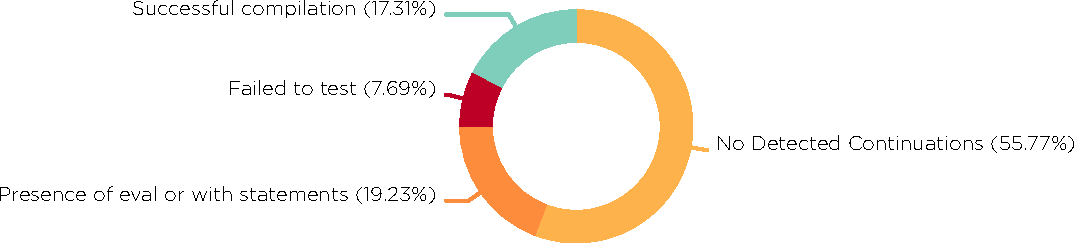
\includegraphics[width=\linewidth]{../resources/due-evaluation.pdf}
  \label{fig:due-evaluation}
  \caption{Results of the Due compiler evaluation}
\end{figure}

On the \num{52} projects composing the test set
\begin{description}
\item[29] (55.77\%) do not contain any compatible continuations,
\item[10] (19.23\%) are not compilable because they contain \texttt{with} or \texttt{eval} statements,
\item[4] (7.69\%) fail their tests before the compilation, and
\item[9] (17.31\%) compile successfully.
\end{description}
The compiler do not fail to compile any project.
The following tables details the results of the evaluation.

29 projects contain no compatible continuation.\\
% \begin{longtabu}{\linewidth}{>{\ttfamily} X r}
\begin{longtabu} to \linewidth {@{} >{\ttfamily\small} X[l] >{\small} r @{}}
\tabucline[.5pt]{-}
app-json-fetcher                      & \comment{release 2.1.0} \\\tabucline[on .5pt]{-}
brokowski                             & \comment{release 0.1.8} \\\tabucline[on .5pt]{-}
claus                                 & \comment{release 0.0.2} \\\tabucline[on .5pt]{-}
code-connect-server                   & \comment{release 0.1.7} \\\tabucline[on .5pt]{-}
costa                                 & \comment{release 0.5.0} \\\tabucline[on .5pt]{-}
csp-endpoint                          & \comment{release 0.0.1} \\\tabucline[on .5pt]{-}
express-device                        & \comment{release 0.3.11} \\\tabucline[on .5pt]{-}
express-resource-plus                 & \comment{release 0.2.1} \\\tabucline[on .5pt]{-}
fizzbuzz-hypermedia-server            & \comment{release 0.1.2} \\\tabucline[on .5pt]{-}
flair-doc                             & \comment{release 0.1.0} \\\tabucline[on .5pt]{-}
generator-wikismith                   & \comment{release 0.2.2} \\\tabucline[on .5pt]{-}
glsl-transition-minify                & \comment{release 0.3.1} \\\tabucline[on .5pt]{-}
heroku-proxy                          & \comment{release 2.1.1} \\\tabucline[on .5pt]{-}
http-test-servers                     & \comment{release 0.0.12} \\\tabucline[on .5pt]{-}
jellyjs-plugin-httpserver             & \comment{release 0.0.8} \\\tabucline[on .5pt]{-}
loopback-angular-cli                  & \comment{release 1.1.1} \\\tabucline[on .5pt]{-}
loopback-explorer                     & \comment{release 1.6.4} \\\tabucline[on .5pt]{-}
moby                                  & \comment{release 1.1.1} \\\tabucline[on .5pt]{-}
monami                                & \comment{release 0.0.21} \\\tabucline[on .5pt]{-}
mongoose-epxress-resource             & \comment{release 0.1.2} \\\tabucline[on .5pt]{-}
nodebootstrap-server                  & \comment{release 1.1.2} \\\tabucline[on .5pt]{-}
oauth-express                         & \comment{release 0.0.1} \\\tabucline[on .5pt]{-}
public-server                         & \comment{release 2.0.1} \\\tabucline[on .5pt]{-}
scrapit                               & \comment{release 0.0.4} \\\tabucline[on .5pt]{-}
sik                                   & \comment{release 0.0.1} \\\tabucline[on .5pt]{-}
sonea                                 & \comment{release 0.0.3} \\\tabucline[on .5pt]{-}
squirrel-server                       & \comment{release 0.0.1} \\\tabucline[on .5pt]{-}
vsoft-explorer                        & \comment{release 0.2.1} \\\tabucline[on .5pt]{-}
webs-weeia                            & \comment{release 0.2.2} \\\tabucline[.5pt]{-}
\end{longtabu}

10 projects contain \texttt{eval} or \texttt{with} statements.\\
\begin{longtabu} to \linewidth {@{} >{\ttfamily\small} X[l] >{\small} r @{}}
\tabucline[.5pt]{-}
adnoce                                & \comment{release 1.1.2} \\\tabucline[on .5pt]{-}
arkhaios                              & \comment{release 0.2.0} \\\tabucline[on .5pt]{-}
browserman                            & \comment{release 0.1.2} \\\tabucline[on .5pt]{-}
infectwit                             & \comment{release 0.0.1} \\\tabucline[on .5pt]{-}
ldapp                                 & \comment{release 0.1.4} \\\tabucline[on .5pt]{-}
levelhud                              & \comment{release 0.1.3} \\\tabucline[on .5pt]{-}
manet                                 & \comment{release 0.3.2} \\\tabucline[on .5pt]{-}
solid                                 & \comment{release 0.2.1} \\\tabucline[on .5pt]{-}
swac                                  & \comment{release 0.12.1} \\\tabucline[on .5pt]{-}
swac-odm                              & \comment{release 0.2.1} \\\tabucline[.5pt]{-}
\end{longtabu}

% 5 projects already use asynchronous frameworks.\\
% \begin{longtabu} to \linewidth {@{} >{\ttfamily\small} X[l] >{\small} r @{}}
% \tabucline[.5pt]{-}
% boomerang-server       & es6-promise  & \comment{release 0.0.1} \\\tabucline[on .5pt]{-}
% hyper.io               & when         & \comment{release 0.2.0} \\\tabucline[on .5pt]{-}
% lanetix-microservice   & bluebird     & \comment{release 1.4.6} \\\tabucline[on .5pt]{-}
% librarian              & bluebird     & \comment{release 1.1.1} \\\tabucline[on .5pt]{-}
% webtasks               & subtask      & \comment{release 0.0.3} \\\tabucline[.5pt]{-}
% \end{longtabu}

4 projects fail their tests before the compilation.\\
\begin{longtabu} to \linewidth {@{} >{\ttfamily\small} X[l] >{\small} r @{}}
\tabucline[.5pt]{-}
express-orm-mvc                       & \comment{release 1.1.0} \\\tabucline[on .5pt]{-}
derpjs                                & \comment{release 0.2.2} \\\tabucline[on .5pt]{-}
hangout                               & \comment{release 0.0.3} \\\tabucline[on .5pt]{-}
ord.zeke.xxx                          & \comment{release 1.0.0} \\\tabucline[.5pt]{-}
\end{longtabu}

% 3 projects do not provide tests.\\
% \begin{longtabu} to \linewidth {@{} >{\ttfamily\small} X[l] >{\small} r @{}}
% \tabucline[.5pt]{-}
% inchi-server                          & \comment{release 0.0.1} \\\tabucline[on .5pt]{-}
% otwo                                  & \comment{release 0.0.1} \\\tabucline[on .5pt]{-}
% tuzi                                  & \comment{release 0.1.5} \\\tabucline[.5pt]{-}
% \end{longtabu}

9 projects successfully compile.\\
\begin{longtabu} to \linewidth {@{} >{\ttfamily\small} X[l] >{\small} r @{}}
\tabucline[.5pt]{-}
express-user-couchdb                  & \comment{release 0.3.5} \\\tabucline[on .5pt]{-}
express-endpoint                      & \comment{release 1.2.11} \\\tabucline[on .5pt]{-}
gifsockets-server                     & \comment{release 0.38.1} \\\tabucline[on .5pt]{-}
heroku-bouncer                        & \comment{release 4.0.1} \\\tabucline[on .5pt]{-}
moonridge                             & \comment{release 0.6.9} \\\tabucline[on .5pt]{-}
redis-key-overview                    & \comment{release 0.0.3} \\\tabucline[on .5pt]{-}
slack-integrator                      & \comment{release 0.0.6} \\\tabucline[on .5pt]{-}
timbits                               & \comment{release 0.7.3} \\\tabucline[on .5pt]{-}
tingo-rest                            & \comment{release 1.0.1} \\\tabucline[.5pt]{-}
\end{longtabu}

The compiler detected 172 callbacks, 52 of them turned out to be compatible continuations.

% \begin{longtabu}{\linewidth}{>{\ttfamily} X r r r r r r }

\begin{longtabu} to \linewidth {@{} X[l] r r r r r r @{}}
\small
                                      & \multicolumn{2}{c}{continuations}      & \multicolumn{4}{c}{chains length}\\
name                                  & total              & compiled          & 1  & 2 & 3 & 4 \\
\tabucline[.5pt]{-}
\texttt{express-user-couchdb}         & 40                 & 20                & 9  & 2 & 1 & 1 \\\tabucline[on .5pt]{-}
\texttt{express-endpoint}             & 19                 & 2                 & 2              \\\tabucline[on .5pt]{-}
\texttt{gifsockets-server}            & 3                  & 1                 & 1  &           \\\tabucline[on .5pt]{-} 
\texttt{heroku-bouncer}               & 7                  & 3                 & 3  &           \\\tabucline[on .5pt]{-}
\texttt{moonridge}                    & 37                 & 6                 & 2  & 2         \\\tabucline[on .5pt]{-}
\texttt{redis-key-overview}           & 14                 & 9                 & 6  &   & 1     \\\tabucline[on .5pt]{-}
\texttt{slack-integrator}             & 6                  & 3                 & 1  & 1         \\\tabucline[on .5pt]{-}
\texttt{timbits}                      & 34                 & 8                 & 8              \\\tabucline[on .5pt]{-}
\texttt{tingo-rest}                   & 12                 & 4                 & 4              \\
\tabucline[.5pt]{-}
total                                 & 172                & 54                & 36 & 5 & 2 & 1 \\
\tabucline[.5pt]{-}
\end{longtabu}

In the following tables, are the name of the callee for each continuations, grouped by package.

% \begin{longtabu}{\linewidth}{>{\ttfamily} X |  l}
\begin{longtabu} to \linewidth {@{} >{\ttfamily} X[l] >{\ttfamily} l @{}}
\tabucline[.5pt]{-}
\multirow{2}{*}{express-endpoint}%
                                      & \texttt{ruleFn} \\
                                      & \texttt{parseParams} \\
% \multicolumn{2}{c}{}\\
\tabucline[on .5pt]{-}
\multirow{9}{*}{express-user-couchdb}%
                                      & \texttt{config.validateUser} \\
                                      & \texttt{createSession} \\
                                      & \texttt{db.destroy} \\
                                      & \texttt{db.get} \comment{$\times5$}\\
                                      % & \texttt{db.get} \\
                                      % & \texttt{db.get} \\
                                      % & \texttt{db.get} \\
                                      % & \texttt{db.get} \\
                                      & \texttt{db.insert} \comment{$\times5$}\\
                                      % & \texttt{db.insert} \\
                                      % & \texttt{db.insert} \\
                                      % & \texttt{db.insert} \\
                                      % & \texttt{db.insert} \\
                                      & \texttt{db.view} \comment{$\times3$}\\
                                      % & \texttt{db.view} \\
                                      % & \texttt{db.view} \\
                                      & \texttt{getUserName} \\
                                      & \texttt{lookupUser} \\
                                      & \texttt{req.session.destroy} \comment{$\times2$}\\
                                      % & \texttt{req.session.destroy} \\
% \multicolumn{2}{c}{}\\
\tabucline[on .5pt]{-}
\multirow{1}{*}{gifsockets-server}%
                                      & \texttt{getRawBody} \\
% \multicolumn{2}{c}{}\\
\tabucline[on .5pt]{-}
\multirow{3}{*}{heroky-bouncer}%
                                      & \texttt{ensureValidToken} \\
                                      & \texttt{oauth.getOAuthAccessToken} \\
                                      & \texttt{request.post} \\
% \multicolumn{2}{c}{}\\
\tabucline[on .5pt]{-}
\multirow{5}{*}{moonridge}%
                                      & \texttt{doc.remove} \\
                                      & \texttt{doc.save} \\
                                      & \texttt{model.findById} \comment{$\times2$}\\
                                      % & \texttt{model.findById} \\
                                      & \texttt{mongoose.connect} \\
                                      & \texttt{populateWithClientQuery} \\
% \multicolumn{2}{c}{}\\
\tabucline[on .5pt]{-}
\multirow{6}{*}{redis-key-overview}%
                                      & \texttt{exec} \comment{$\times2$}\\
                                      % & \texttt{exec} \\
                                      & \texttt{execstderr} \\
                                      & \texttt{fs.unlink} \\
                                      & \texttt{fs.writeFile} \comment{$\times2$}\\
                                      % & \texttt{fs.writeFile} \\
                                      & \texttt{request.post} \\
                                      & \texttt{res.sendfile} \comment{$\times3$}\\
                                      % & \texttt{res.sendfile} \\
                                      % & \texttt{res.sendfile} \\
% \multicolumn{2}{c}{}\\
\tabucline[on .5pt]{-}
\multirow{3}{*}{slack-integrator}%
                                      & \texttt{config.payload} \\
                                      & \texttt{sendPayload} \\
                                      & \texttt{request} \\
% \multicolumn{2}{c}{}\\
\tabucline[on .5pt]{-}
\multirow{5}{*}{timbits}%
                                      & \texttt{loadTimbits} \\
                                      & \texttt{res.render} \\
                                      & \texttt{timbit.test} \comment{$\times2$}\\
                                      % & \texttt{timbit.test} \\
                                      & \texttt{timbits.pantry.fetch} \comment{$\times2$}\\
                                      % & \texttt{timbits.pantry.fetch} \\
                                      & \texttt{request} \\
% \multicolumn{2}{c}{}\\
\tabucline[on .5pt]{-}
\multirow{4}{*}{tingo-rest}%
                                      & \texttt{req.collection.findOne} \\
                                      & \texttt{req.collection.insert} \\
                                      & \texttt{req.collection.update} \\
                                      & \texttt{req.collection.remove} \\
\tabucline[.5pt]{-}
\end{longtabu}{}


















% Tested applications :

% rest-api-express            -> OK

% socket-testing              -> OK (partial) the project is broken, but it seems broken in the same way before and after the compilation :)
% nodeExample                 -> OK (partial) read-simple.js and write-simple.js compile successfully (the only two files to contain continuation). but the project compiler breaks, I suspect it is because of some !# stuffs. 

% fligg                       -> NOK not functionnal : impossible to log, or sign in
% colors                      -> NOK no continuations
% request                     -> NOK no continuations=:
% async                       -> NOK presence of with or eval
% penguin                     -> NOK not functionnal : syntax error
% expression.io               -> NOK tests not passed before compilation

% blog-experiment             -> NOK already use thenable



% NPM

% app-json-fetcher              -> NOK no continuations
% express-resource-plus         -> NOK no continuations
% fizzbuzz-hypermedia-server    -> NOK no continuations
% flair                         -> NOK no continuations
% generator-wikismith           -> NOK no continuations
% brokowski                     -> NOK no continuations
% claus                         -> NOK no continuations
% costa                         -> NOK no continuations
% express-device                -> NOK no continuations
% heroku-proxy                  -> NOK no continuations
% http-test-servers             -> NOK no continuations
% jellyjs-plugin-httpserver     -> NOK no continuations
% loopback-angular-cli          -> NOK no continuations
% loopback-explorer             -> NOK no continuations
% monami                        -> NOK no continuations
% mongoose-epxress              -> NOK no continuations
% nodebootstrap-server          -> NOK no continuations
% oauth-express                 -> NOK no continuations
% public-server                 -> NOK no continuations
% scrapit                       -> NOK no continuations
% sik                           -> NOK no continuations
% sonea                         -> NOK no continuations (coffee)
% vsoft-explorer                -> NOK no continuations
% webs-weeia                    -> NOK no continuations
% code-connect-server           -> NOK no continuations
% csp-endpoint                  -> NOK no continuations
% glsl-transition-minify        -> NOK no continuations
% moby                          -> NOK no continuations
% squirrel-server               -> NOK no continuations
%   >> 29 no continuations

% arkhaios                      -> NOK presence of with or eval
% browserman                    -> NOK presence of with or eval
% infectwit                     -> NOK presence of with or eval
% ldapp                         -> NOK presence of with or eval
% levelhud                      -> NOK presence of with or eval
% manet                         -> NOK presence of with or eval
% solid                         -> NOK presence of with or eval
% swac                          -> NOK presence of with or eval
% swac-odm                      -> NOK presence of with or eval
% adnoce                        -> NOK presence of with or eval
%   >> 10 with or eval

% boomerang-server              -> NOK already use thenable (es6-promise)
% hyper.io                      -> NOK already use thenable (when)
% node-lanetix-microservice     -> NOK already use thenable (bluebird)
% librarian                     -> NOK already use thenable (bluebird)
% webtasks                      -> NOK already use async stuffs (subtask)
%   >> 5 async frameworks

% xtc                           -> NOK unexpected token < use templating engine to generate js@
% agenda-ui                     -> NOK unexpected reserved word use ES6 specifications
% traffic-light                 -> NOK illegal return statement
% ellipsis                      -> NOK illegal return statement
%   >> 4 incorrect code

% express-orm-mvc               -> NOK test failed (this project is just a template)
% hangout                       -> NOK test failed (unfinished ?)
% derp                          -> NOK test failed + this project use generators
% ord                           -> NOK however test failed similarly after and before compilation
%   >> 4 test failed

% tuzi                          -> NOK no tests
% inchi-server                  -> NOK no tests
% otwo                          -> NOK no tests
%   >> 3 no tests

% to compile
% express-couchUser             >> 13 chains (20 continuations / 40)   1: 9,      2: 2,      3: 1,      4: 1
% gifsockets-server             >> 1 chains (1 continuation / 3)       1: 1
% node-heroku-bouncer           >> 3 chains (3 continuations / 7)      1: 3
% moonridge ( +install morgan)  >> 4 chains (6 continuations / 37)     1: 2      2: 2
% redis-key-overview            >> 7 chains (9 continuations / 14)     1: 6                  3: 1
% slack-integrator              >> 2 chains (3 continuations / 6)      1: 1      2: 1
% timbits                       >> 8 chains (8 continuations / 34)     1: 8
% tingo-rest                    >> 4 chains (4 continuations / 12)     1: 4
% express-endpoint              >> 2 chains (2 continuations / 19)     1: 2 and already use async stuffs (step)
%   >> 9 OK total of 56 continuations / 172, 1:36 2:5 3:2 4:1


% 29 no continuations
% 10 with ot eval
% 5 async
% 4 incorrect code
% 4 test failed
% 3 no tests
% 9 OK

% total 64 Projects